\documentclass{acm_proc_article-sp}[12pt]
\usepackage{cite}
\usepackage[english]{babel}
\usepackage{listings}
\usepackage{subfigure}
\usepackage{url}
\lstset{language=C,
       basicstyle=\small,
       numbers=left,
       stepnumber=1,
       numbersep=5pt,
       commentstyle=\color{red},
       escapeinside={(*@}{@*)}}

%%%%%%%%%%%%%%%
% Commenting on the paper:
%%%%%%%%%%%%%%%%%
\definecolor{midblue}{rgb}{0.7,0.9,1}
\definecolor{orange}{rgb}{1,0.9,0.6}
\definecolor{lightgreen}{rgb}{0.6,1,0.6}
\definecolor{grey}{rgb}{0.9,0.9,0.9}

\newcommand{\comment}[2]{\begin{center}\colorbox{#1}{\parbox{0.85\linewidth}{\textit{{#2}}}}\end{center}}

\newcommand{\abdullah}[1]{\comment{midblue}{{Abdullah: #1}}}
\newcommand{\lauro}[1]{\comment{orange}{{Lauro: #1}}}
\newcommand{\elizeu}[1]{\comment{lightgreen}{{Elizeu: #1}}}
\newcommand{\matei}[1]{\comment{grey}{{Matei: #1}}}

%\title{Totem: Massively-Parallel Graph Processing Framework}
\title{Massively-Parallel Graph Processing}
\numberofauthors{1}
\author{
% 1st. author
\alignauthor 
Lauro Beltr\~ao Costa, Abdullah Gharaibeh, Elizeu
Santos-Neto\vspace{3mm}\\
       \affaddr{\small{University of British Columbia}}\\
       \affaddr{\small{2332 Main Mall, Vancouver, BC, CANADA}}\\
       \email{\small{\{lauroc,abdullah,elizeus\}@ece.ubc.ca}}
}
\date{ January 2011}

\begin{document}

\maketitle

%\abdullah{Comments by Abdullah}
%\lauro{Comments by Lauro}
%\elizeu{Comments by Elizeu}

\begin{abstract}
The goal of this project is to understand the challenges in porting graph algorithms to multi-core architectures. In particular, this work focuses on hybrid massively-parallel platforms that consist of processors optimized for sequential processing and accelerators optimized for massively-parallel processing. Understanding the design and implementation of a range of graph algorithms is the first step towards building a generic graph processing framework on such architectures.

To this end, we study a number of graph algorithms such as breadth-first search, single source shortest path, and PageRank. We focus on algorithms that are in the core of many relevant applications such as social network analysis, web search, transportation routes, paths of disease outbreaks, and citations among scientific papers.

This work presents the first step towards designing {\sc Totem} -- a graph-processing framework that leverages massively parallel hybrid platforms. In particular, we give implementations of core graph algorithms (i.e., BFS, Dijkstra's algorithm, and PageRank) and preliminary performance analysis of some of these algorithms. Also, we discuss the future work based on the current experience provided by these initial implementations.


\end{abstract}

% A category with the (minimum) three required fields
%\category{H.4}{Information Systems Applications}{Miscellaneous}
%A category including the fourth, optional field follows...
%\category{D.2.8}{Software Engineering}{Metrics}[complexity measures, performance measures]
%\terms{Theory}
%\keywords{ACM proceedings, \LaTeX, text tagging} % NOT required for Proceedings

\section{Introduction}
Graphs are everywhere. From the nowadays omnipresent online social networking tools to the structure of fundamental scientific problems, passing through mundane applications such as finding the best bicycle route between two points in a city, graphs are indeed a building block to model several important problems.

However, the scale of current graphs calls for new computational platforms and techniques that support efficient processing. Currently, two main platforms are common: on the one end, high-performance, yet expensive and specialized supercomputers such as Cray machines have been deployed~\cite{mizell2009early, yoo2005scalable}; on the other end, less efficient, yet commodity and expandable traditional clusters are also being used in production systems~\cite{Malewicz2009}. Between these two ends, hybrid commodity platforms (e.g., GPU-supported clusters) have the potential to offer the good of two platforms: a high-performance, low-cost system.

To this end, this work investigates the general challenges of processing graph algorithms on hybrid commodity systems (e.g., GPU-supported clusters). Additionally, in the spirit of building abstractions to hide complexity, the ultimate goal is to build a generic graph-processing framework that leverages massively-parallel hybrid platforms. In particular, this work aims at addressing the following questions:

\begin{enumerate}
\item What are the general challenges to support graph processing on a hybrid, GPU-based compute node? Is it possible to partition the processing to efficiently use both the main processor and the GPU? In other words, given a fixed die area or power budget, is it more efficient to rely on a traditional symmetric multi-processor (SMP) or a hybrid node?

\item Assuming that a hybrid, GPU-based node brings performance benefits, is it efficient to use a GPU-supported cluster to process large-scale graph problems compared to a traditional cluster? In other words, in a traditional cluster setup, is the computation phase dominant enough compared to the communication phase such that adding a massively-parallel component to speedup the computation phase would improve the end-to-end system performance?

\item Assuming that graph algorithms can efficiently leverage GPU-supported clusters, what should a graph processing framework that aims at simplifying the task of implementing graph algorithms on such platforms provide to developers? Specifically, what is the adequate parallel processing model (e.g., BSP - Bulk Synchronous Processing~\cite{Valiant1990}, PRAM~\cite{Fortune78}, or LogP~\cite{Culler1996}), graph-level abstractions (e.g., vertex or edge centric), and the high-level interface of a sufficiently expressive, yet performance-efficient framework?

\item Hiding complexity and problem-specific optimizations are often conflicting goals: a framework that reduces complexity may mask hardware details that could be used to optimize specific graph algorithms. With this in mind, what is the performance cost generated by introducing an abstraction layer between the graph algorithms and the hardware platform?

\item Ultimately, a graph-processing framework should enable measurable gains from the application standpoint. Thus, can we identify applications (e.g., PageRank) where the use of such framework enables problem-solving at larger scales or faster than current platforms?

\end{enumerate}

At this stage, we report on our progress towards addressing the first question. We present preliminary performance results for a number of graph algorithms on a single GPU and compare them with high-end SMP systems. We show that graph algorithms are memory-latency bound, and that traditional SMP systems are not optimized to support such a processing pattern. We also show that a GPU can offer important performance speedups due to its ability to hide memory access latency through massive multithreading.

The next sections present the opportunities, goals, and anticipated challenges of this project (\S~\ref{sec:motivation}); related work (\S~\ref{sec:related}); methodology (\S~\ref{sec:methodology}); current progress (\S~\ref{sec:progress}); future work (\S~\ref{sec:future}); and, concluding remarks (\S ~\ref{sec:conclusion}).

\section{Related Work}
\label{sec:related}

\elizeu{This section is the same as in the 571R final report.}

This project spans the following areas: graph algorithms, in general, and parallel graph algorithms, in particular; graph algorithms on GPUs; and parallel graph processing frameworks. This section briefly positions this work among the related literature.

{\bf Parallel graph algorithms.} Although graph algorithms are a well studied area, leveraging parallel architecture to accelerate the algorithm runtime is far from a straightforward task. A parallel implementation may require substantial changes to the original sequential algorithm and strong assumptions about the parallel platform. The required changes and assumptions come at the expense of making the algorithm less portable across platforms. Sometimes, graph problems that have optimal sequential algorithms, dlack a optimal parallel counterpart (e.g., Dijkstra's algorithm is a provably optimal sequential algorithm for the single source shortest path, but an optimal parallel algorithm for this problem is unknown).  

Although the PRAM~\cite{Fortune78} parallel processing model is vastly used in the study of parallel algorithms~\cite{Quinn1984,Atallah1984}, some recent works try to provide performance analysis on distributed memory machines models. Meyer and Sanders~\cite{Meyer2003}, for example, gives a parallel algorithm for single source shortest path named $\Delta$-stepping. The authors analyze the performance of the algorithm in the PRAM model and provide extensions to distributed memory model. The algorithm works by keeping nodes with tentative distances in separate buckets where each bucket represent the distances within the range of size $\Delta$. In each phase, the algorithm consider the nodes in the non-empty buckets and edges of weight up to $\Delta$. Parallelism is achieved by processing the nodes in a given bucket concurrently. 

{\bf Graph algorithms on GPUs.} Previous work investigates the use of GPUs to accelerate graph computation~\cite{Harish2007, Katz2008, Sungpack2010, dehne2010exploring}. For example, Sungpack et al.~\cite{Sungpack2010} shows that, in the case of breadth-first search, a single Nvidia Tesla GPU offers up to 2.5x speedup compared to dual socket, quad-core Intel Xeon symmetric multiprocessor on realistic workloads. However, those works focus on few graph algorithms, mainly breadth-first search, single source shortest path, and all pairs shortest path. Moreover, the implementations assume that the graph fits GPU memory, which puts a limitation on the size of graphs that can be processed. 

A natural scaling path is to run large graph algorithms into multi-GPU systems. Katz et al.~\cite{Katz2008} implement a hand-crafted version of all pairs shortest path algorithm for multi-GPU systems. However, the proposed approach is tightly coupled with the problem and cannot be generalized to other algorithms. Additionally, the implementation provided by Katz et al. assumes an adjacency matrix graph representation that imposes a significant space overhead for sparse graphs, a characteristic that is common in the majority of real-world graphs. Yet another, nevertheless fundamental, challenge to harness multi-GPU systems is to adapt these algorithms from the PRAM model to a distributed memory machines model such as BSP or LogP. Gerbessiotis and Valiant provide results on the performance impact on emulating a DMM model with PRAM~\cite{Gerbessiotis92}. 

{\bf Graph processing frameworks.} The Parallel BGL~\cite{gregor2005parallel} and Pregel~\cite{Malewicz2009} present frameworks to implement distributed graph algorithms. Both frameworks specify generic concepts for designing distributed graph algorithms. The frameworks are based on abstractions that are common among graph algorithms. Examples of such abstractions include vertices, edges, property maps {\em (key-value pairs)}, and mechanisms for data propagation and graph traversal. 

It is worth noting that PBGL, Pregel, and others~\cite{Zhao2009} assume traditional cluster systems (i.e., nodes connected via network and containing traditional multi-core processors). This work targets, on the other hand, hybrid GPU-based systems, which have different computational model and offer different trade-offs and challenges. 

To the best of our knowledge, there is no graph processing framework optimized for hybrid GPU-based platforms. A framework specialized for GPU-based platforms could minimize communication overhead over the GPU's high-latency I/O channels (e.g., employing compact messaging and graph representations to minimize communication and space footprint); also it could offer graph-specific abstractions that hide the GPU's complex memory model while efficiently leveraging it (e.g., transparently utilizing shared memory). 

\section{Methodology}
\label{sec:methodology}
The methodology consists of algorithm design, prototyping, and performance analysis (both theoretical and experimental).
The first, and ongoing, step is bibliography review in order to better understand the areas described in \S~\ref{sec:related}, and how they relate to each other. Note that the work discussed in \S~\ref{sec:related} is not an exhaustive list.

The second phase is to port simple, yet well known graph algorithms to GPUs~\cite{Quinn1984,Meyer2003,Harish2007,Malewicz2009,Sungpack2010}). Implementing simple graph algorithms on GPUs gives us familiarity with the algorithms and the platform. Building hands-on expertise on graph problems is an important step towards designing the framework. It will inform what should be the building blocks provided by the framework and how to leverage the platform. Additionally, this step will inform the theoretical analysis of expected peak performance one can achieve on particular graph algorithms when executed on GPU platforms.

The third phase is to assess the value of improving the compute phase when processing graphs on traditional cluster setups. This is done via simple modeling, which will take into account a number of important aspects such as the parallel processing model and the bandwidth and the latency of the various communication links (inter- and intra- node).

Informed by the past steps, the third step will focus on defining building blocks of the graph processing framework, such as the parallel processing model, abstractions, the communication substrate and the high-level interface. Moreover, this phase aims to define the scope of graph algorithms the framework will support. In particular, we need to consider several design trade-offs carefully. Among these design decisions are: Should the framework support directed or undirected edges? should the programming model support vertex- or edge-centric? What is the impact on the class of applications supported? are dynamic changes allowed in the graph? All these questions will help shaping the preliminary design of the graph processing framework.


\section{Progress to Date}
\label{sec:progress}

This section provides a description of the three algorithms implemented (\S~\ref{sec:implementation}) so far and some preliminary evaluation results (\S~\ref{sec:evaluation}). In summary, the work done so far consists of literature review, which is described in the related work section (\S~\ref{sec:related}) and an initial implementation that will serve as the basis for the framework.

\subsection{Implemenation}
\label{sec:implementation}

The largest part of the development infrastructure is ready. This includes a graph file format, graph parser, unit tests, makefiles, code review tool, and code repository. More importantly, we implemented three graph algorithms on the GPU: breadth-first search, single source shortest path, and PageRank. The rest of this section discusses the graph data structure we used, and the implementation of each of the aforementioned algorithms. Note that, for all algorithms, we omit several implementation details (e.g., memory transfers) and we assume that the graph fits GPU memory.

\textbf{Graph data structure.} A graph $G(V,E)$ is represented as an adjacency list by two arrays: vertices and edges. The vertices array stores for each vertex the start position in the edges array of a vertex's outgoing edges. The edges array stores the destination vertices of the outgoing edges. This is a common data structure to represent graphs, and was used in other related work~\cite{Harish2007, Sungpack2010}.

{\bf Breadth-First Search.} Breadth-first search (BFS) traverses the graph in levels given a source vertex; once a level is visited, none of the vertices in that level is visited again. Listing \ref{lst:bfs} presents the implementation of BFS where the goal of transversal search is calculating the distance from a source vertex to every other vertex in the graph; such distances are stored in the cost array. Lines $1-9$ show the function that executes on the CPU: for each level in the graph, it calls the \texttt{bfskernel} to process the vertices in the current level.


\begin{lstlisting}[caption=Breadth-First Search Implementation,label=lst:bfs]
__host__ int*
bfs_gpu(int source_id, graph* g) {
  ...
  for (int level = 0; !finished; level++) {
    finished = true;
    launch_bfs_kernel(g, level, &finished, cost);
  }
  ...
}

__kernel__void
bfs_kernel(graph* g, int level, bool* finished,
           int* cost) {
  int v_id = THREAD_GLOBAL_INDEX;
  if (v_id >= g.vertex_count) return;
  if (cost[v_id] != level) return;

  for (int i = g.vertices[v_id]; 
       i < graph.vertices[v_id + 1]; i++) {
    int nghbr = graph.edges[i];
    if (cost[nghbr] == INF) {
      *finished = false;
      cost[nghbr] = level + 1;
    }
  } // for
}
\end{lstlisting}

Each GPU thread processes a vertex. An integer array, \texttt{cost}, stores the minimal number of edges from the source vertex to each edge. The cost for vertices that have not been visited yet is infinity (INF). In each iteration, each thread checks if its vertex belongs to the current level by verifying the cost in the \texttt{cost} array (line 16). If true, it updates the costs of its not yet visited neighbors (lines $18-25$). If the cost of at least one neighbor is updated, the variable \texttt{finished} is set to \texttt{false} and there will be another iteration. Note that threads may update \texttt{finished} at the same position in the \texttt{cost} array concurrently. Such concurrent access may impact the performance of the implementation, but it does not affect correctness since all threads update the memory with the same value. The iterations are repeated until all the levels are visited.

{\bf Single Source Shortest Path.} In this work, we consider Dijkstra's algorithm that computes the single source shortest paths. Given a weighted undirected graph $G = (V, E, w)$ and a source node $s \in V$, the algorithm computes the distances from $s$ to every other node in the graph. Listing~\ref{lst:sssp} provides our current {\sc cuda} implementation based on the Dijkstra's algorithm in Harish et al.~\cite{Harish2007}.


\begin{lstlisting}[caption=GPU implementation of Single Source Shortest Path algorithm,label=lst:sssp]
__kernel__
void dijkstra_kernel(graph_t g, bool* mask, 
                     int* distances, 
                     int* new_distances) {
  const int v_id = THREAD_GLOBAL_INDEX;
  if (v_id >= g.vertex_count || !mask[v_id]) {
    return;
  }
  mask[v_id] = false;

  int my_dist = distances[v_id];
  for (int i = g.vertices[v_id]; 
       i < g.vertices[v_id + 1]; i++) {
    int nghbr = graph.edges[i];
    int* new_dist = &(new_distances[nghbr]);
    int cur_dist = my_dist + g.weights[nghbr];
    // avoid race condition
    *new_dist = atomicMin(*new_dist, cur_dist);
  } // for
}
\end{lstlisting}

{\bf PageRank.} Listing \ref{lst:pagerank} presents the implementation of PageRank. For each round, every vertex broadcasts its tentative PageRank divided by the number of outgoing edges. The tentative PageRank of a vertex is calculated as follows: the vertex sums up the value broadcasted by each of its neighbors and sets its own tentative PageRank to $((1 - d) / vertex\_count + d * sum$, where $d$ is the damping factor\footnote{A probability that models the behavior of the random surfer when she moves from one page to another without following the links on the current page.}. Broadcasting messages over outgoing edges is done as follows: the value is placed in the outbox buffer. In the next round, the inbox and outbox buffers are swapped, and the message will be accessed in the next round via the inbox buffer. This operation simulates a broadcast because all the neighbors of vertex $v$ will access the same location (i.e., \texttt{inbox[v]}) to get the message. In the last round, the outbox will contain the PageRank of each vertex. Note that for PageRank, we assume that the edges array stores the incoming edges rather than the outgoing edges.

\begin{lstlisting}[caption=GPU implementation of PageRank,label=lst:pagerank]
__host__ float* 
page_rank_gpu(graph_t* g) {
  ...
  for (int round = 0; round < MAX_ROUNDS;
       round++) {
    // simulate message passing
    float* tmp = in_d;
    in_d = out_d;
    out_d = tmp;
    bool finished = (round == (MAX_ROUNDS - 1));
    launch_page_rank_kernel(g, in_d, out_d,
                            finished);
  }
  ...
}

__kernel__
page_rank_kernel(graph_t g, float* in, 
                 float* out, bool finished) {
  id_t v_id = THREAD_INDEX;
  if (v_id >= g.vertex_count) return;
  // sum the rank of all neighbors
  double sum = 0;
  for (int i = g.vertices[v_id]; 
       i < g.vertices[v_id + 1]; i++) {
    int nghbr = g.edges[i];
    sum += in[nghbr];
  }
  // calculate my rank
  float rank = ((1 - d) / g.vertex_count) +
               (d * sum);
  out[v_id] = finished ?
              rank : rank / nbrs_count;
}
\end{lstlisting}


%\matei{The only substantial comment relates to approach.  Implementations are costly. So I wonder to what degree the use of a simplified execution model could give you some idea about the bounds of the efficiency one could get on a GPU?   (Or the percent of the bottleneck resource your graph parallel algorithm will be able to use?)  This might help you understand the relative speedups provided by GPUs and CPUs (e.g., compred to, let's say one core), and will force you to think about the critical properties of the algorithms you'll try to implement.   I realize what I am suggesting is, with a relatively high probability, a dead-end.  However, if it does go somewhere it will save a lot of  time.}

\elizeu{I added a new reference that discusses the impact on performance by moving from a PRAM to DMM model. This might be useful to understand the impact on parallel algorithms in multi-gpu cases.}

All the rest are minor comments:

\matei{(in section 3): I would de-emphasize the framework - this is too ambitious in my opinion. At this point your goal is a feasibility study.}

\abdullah{I disagree here with Matei, also it is not clear to me whether we can actually do a good enough feasibility study, I think we have enough indication from previous work that graphs on GPU could work.}

\elizeu{I agree with Abdullah. I think we reached a good middleground. I kept the discussion about the framework as a goal. But, led the discussion towards the first steps we are taking.}

\matei{Would a critical look at past implementations of graph algorithms for GPUs be useful?  I guess this is implicit when you say "The second phase is to port simple, yet well known graphs algorithms to GPUs [5, 8, 9, 14])."}

\abdullah{we should discuss in the related work section: BSP model in Pregel, virtual warp concept}

\elizeu{I added extra discussion in the related work about the considered models, perhaps we can expand later}

\matei{Can you provide a clearer delineation for the class of graph problems you are interested in? By scale? By complexity of algorithm?}

\abdullah{traversal algorithms in general?}

\elizeu{So, far I'd say that traversal has been the focus: 2 out of the three algorithms. But, overall we want a more diverse mix, I think we can discuss the classes of algorithms later.}



\subsection{Performance Evaluation}
\label{sec:evaluation}

This section presents preliminary performance evaluation of the algorithms described in the previous section, and workload characterization. The goal is to provide insights into the attainable graph processing performance on accelerators, and to understand the characteristics of graph workloads that impact the observed performance. 

In particular, the experiments focus on the processing rate (i.e., edges / sec) of the three implementations of {\sc bfs}, Dijkstra, and PageRank: sequential, multi-threaded, and GPU. The workload is composed of both synthetic and real-world graphs\footnote{\url{http://snap.stanford.edu/data/}}. Table~\ref{tab:workload} summarizes the workloads. The synthetic graphs are generated by the R-MAT~\cite{rmat} tool and provides a reference point of comparison to other studies in the parallel graph processing literature~\cite{agarwal2010scalable}.

R-MAT (Recursive MATrix) \cite{rmat} is a method to generate power-law graphs given few parameters. Its input is the number of nodes, number of edges, and four values ($a$, $b$, $c$, and $d$) that represent probabilities. R-MAT creates an adjacency matrix, divides it into four partitions of equal size, and associates each of the input probabilities to a partition. To create an edge, R-MAT selects one of the partitions according to their assigned probabilities. The chosen partition is divided again into four smaller partitions, and the procedure is repeated until a partition of $1 \times 1$ (a single cell) is left, in which an edge is created. When $(a : b) = (a : c) \approx 3$ and $a > d$, the generated graph is a power-law graph. The relation $a : d$ also controls the skewness of the node degree distribution in the generated graph.

\begin{table}[ht]
\centering
\begin{tabular}{l|r|r|c}
Name              & $|V|$   & $|E|$      & Directed \\\hline
Web (Google)      & 875,713 & 5,105,039  & yes      \\\hline
Web (NotreDame)   & 325,729 & 1,497,134  & yes      \\\hline
Web (Stanford)    & 281,903 & 2,312,497  & yes      \\\hline
OSN (LiveJournal) & 4,847,571 & 68,993,773 & yes    \\\hline
A45         & 10,000,000 & 49,998,874 & no \\\hline
A4          & 10,000,000 & 49,999,826 & no \\\hline
A59         & 10,000,000 & 49,339,676 & no \\\hline
A6          & 10,000,000 & 49,477,202 & no \\\hline
\end{tabular}
\caption{Graphs used in the experiments.}
\label{tab:workload}
\end{table}

We evaluate the implementation of the algorithms on a machine with dual-socket Intel Xeon Quad-core processor (E5520 @ 2.27GHz), and 16GB of system memory. The GPU installed on the machine is an NVIDIA GeForce GTX 480: 480 cores clocked at 1400MHz, and has 1536 MB memory. The results that follow compare the processing rate of three implementations of each algorithm: sequential CPU, multi-threaded CPU (using OpenMP with 128 threads), and a GPU implementation.

\begin{figure*}[ht]
\begin{center}
\mbox{\scalebox{1}{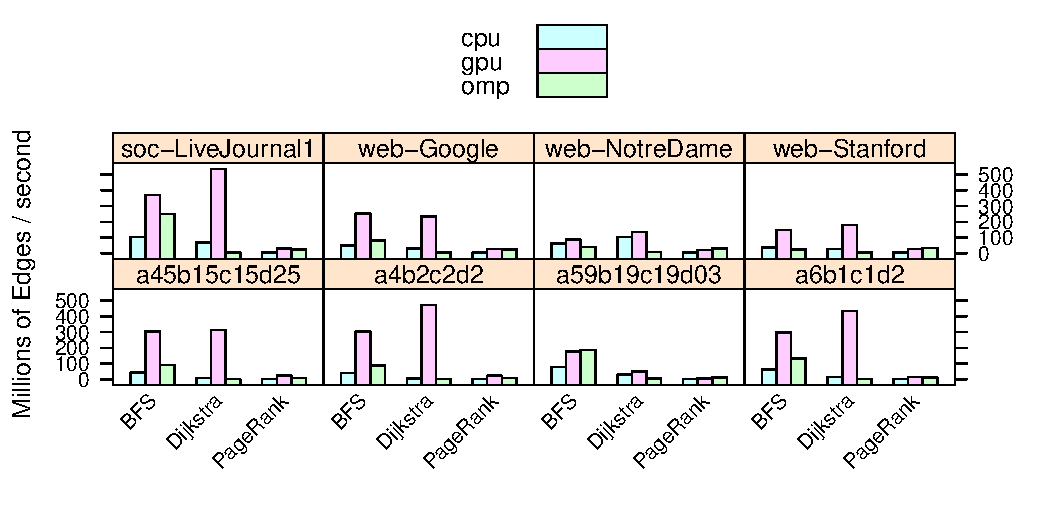
\includegraphics{figures/edges_per_second.pdf}}}
\caption{Processing rate}
\label{fig:rate}
\end{center}
\end{figure*}

Figure \ref{fig:rate} shows the processing rate (i.e., edges per second) for each combination of algorithm, workload, and platform. There are two important aspects to highlight. First, the GPU implementation achieves superior performance in the majority of scenarios; second, the observed performance variation from one scenario to another suggests that graph characteristics play an important role in the attainable performance. The next paragraphs discuss these points in turn.

In the set of real-world graphs (top line), the GPU implementation achieves a peak performance of approximately $372$ millions of edges per second (BFS, LiveJournal). It is important to note that this is an estimation of the processing rate an accelerator (in a hybrid system) would be able to deliver compared to alternative platforms. In practice, the GPU would be primarily used to offload processing from the host processors. Therefore, such hybrid platform has the potential to deliver even higher performance when compared to the referred CPU and OpenMP implementations evaluated above.

Although the performance levels above provide evidence that hybrid platforms are attractive for graph processing, we also observe some variations in the relative performance across workloads for the same algorithm. More specifically, the relative performance of PageRank on GPU and OpenMP platforms seems to depend on the workload. This is illustrated by the processing rates achieved on {\em web-Google} and {\em liveJournal} compared to {\em web-NotreDame} and {\em web-Stanford}. Similarly, the relative performance is not consistent across the R-MAT graphs. 

One potential source for these inconsistencies is the work imbalance across threads, which is a result of non-uniform connectivity across the nodes in the graph (e.g., node degree). More specifically, the hypothesis is that node degree imbalance will cause thread divergence in the GPU-implementations and hinder its performance. 

To test this hypothesis, we characterize the node degree distribution of each graph in the workload and correlate it with the achieved performance. The characterization considers two metrics of the concentration of a distribution: Kurtosis, a measure of the "peakedness" of the node degree distribution; and the $\alpha$ coefficient of a fitted power-law (i.e., the slope of the line on the log-log plot of the node degree distribution) (see Table~\ref{tab:kurtosis}). 

\begin{table}[ht]
\centering
\begin{tabular}{l|r|r}
Name              & Kurtosis   & $\alpha$ \\\hline
Web (Google)      & 142.20   & 1.47    \\\hline
Web (NotreDame)   & 2088.50  & 1.45    \\\hline
Web (Stanford)    & 57.60    & 1.45    \\\hline
OSN (LiveJournal) & 29667.00 & 1.40    \\\hline
A45               & 132.02  & 1.51    \\\hline
A4                & 167.50   & 1.51    \\\hline
A59               & 73959.00 & 1.56    \\\hline
A6                & 3660.10  & 1.55     \\\hline
\end{tabular}
\caption{Approximate values for the node degree distribution characteristics metrics.}
\label{tab:kurtosis}
\end{table}
            
If there is a negative correlation between the characteristics of the node degree distribution, as represented by the kurtosis and the $\alpha$ coefficient, the influence of the node degree distribution imbalance on the performance is confirmed. 

\begin{table}[ht]
\centering
\begin{tabular}{l|r|r}
Name     & $\rho(kurtosis,e)$ & $\rho(\alpha,e)$ \\\hline
BFS      & -0.2049       &  0.2649 \\\hline
Dijkstra & -0.5921       & -0.0869 \\\hline
PageRank & {\bf -0.6632} & {\bf -0.7331} \\\hline
\end{tabular}
\caption{Person's correlation coefficient between processing rate of GPU implementations and the workload characteristics.}
\label{tab:corr}
\end{table}

Table~\ref{tab:corr} contains the the Person's correlation coefficient $\rho$ between the observed performance (i.e., edges/s $= e$) of each GPU implementation and the workload characteristics. These results confirm our intuition that the inconsistencies in performance observed on the GPU implementation of PageRank is due to relatively few high-degree nodes. The existence of these nodes translate into a {\em peaky} node degree distribution (i.e., a large value for both $\alpha$ and kurtosis). In turn, such graph workload imply less parallelism in the application, as some threads will have much more work to process, while others finish early and stay idle. 

Although these correlations provide initial support to the intuition that the node degree distribution characteristics influence the observed performance of graph algorithms on GPU, these results should be taken with caution. A more comprehensive study that includes a larger sample of both real-world and synthetic graphs together with the application of complementary data analysis approaches (e.g., regression analysis, and principal component analysis) is necessary to provide a statistically grounded conclusion. Nevertheless, these preliminary results show that we are on the right direction.

Finally, it is worth noting the poor performance of the OpenMP implementation of Dijkstra's algorithm: the processing rate is consistently lower than that for its sequential version. The reason for this bad performance is granted to a naive synchronization approach adopted in the current OpenMP implementation. Threads use a global lock over the entire set of vertices, when only a lock that protects only the neighbors of a given vertex that are processed by the current thread. A simple solution that trades run time for a larger memory footprint consists of having one lock per vertex in the graph. The evaluation of such implementation is left for future work.

\section{Future Work}
\label{sec:future}

Implementing {\sc bfs}, Dijkstra's and PageRank algorithms already helped to identify the commonalities among graph algorithms. For example, operations that sweep through the list of neighbors of each vertex are present in all three algorithms. Therefore, defining common building-block kernels that can be used by a variety of graph algorithms is clearly a potential way to go. Additionally, and equally important, there are logistics operations such as graph parsing and initialization, memory allocation, and data transfer routines that can also be part of an infrastructure shared by all the algorithms. In fact, some of these operations are already provided as abstractions in the current version of {\sc totem}.

Besides the abstractions that are undoubtedly useful in single-GPU hybrid platforms, it is also necessary to study and design new abstractions for a multi-GPU environment. To this end, we will first investigate the potential losses in performance due to the mismatch between the parallel programming model assumed by the algorithms (i.e., PRAM) and the model that best match a multi-GPU platform (e.g., BSP). This effort can benefit from previous studies on the translation of parallel algorithms from on model to another~\cite{Gerbessiotis92}. 

It is also important to show benefits at the application layer. Therefore, we consider a list of candidate applications that could provide evidence of {\sc Totem}'s applicability and good estimates of the application-level performance that {\sc Totem} can deliver. 

{\bf Community detection.} Online social systems are commonplace nowadays. Graphs are unsurprisingly the mathematical abstraction of choice to study the characteristics of user interactions in these systems. One important application is the detection of subgroups of users where the connections are stronger within the group than those to individuals outside the group. This application is called {\em community detection}. The scale of existing social networks demands efficient and scalable solutions for community detection. This application is a good candidate as it may build upon the already implemented algorithms (e.g., Girwan-Newman's community detection algorithm~\cite{Newman2004} which is based on a centrality measure that uses {\sc bfs}).

{\bf Characterization of time-evolving social networks.} Although online social networks are inherently dynamic (i.e., users are actively exchanging public/private messages, producing and consuming content), the vast majority of studies that analyze such network focus on static snapshots of the network~\cite{Willinger2009}, specially due to the computational cost of analysing large networks while considering their time-evolving characteristics. Thus, we plan to use {\sc Totem} to enable the characterization of structural aspects of dynamic online social networks. In particular, we focus on the following question: what is the rate of variation in node centrality measures in a network with time-evolving edge weights? This study can also leverage already implemented algorithms by extending them to compute centrality measures efficiently.

Finally, the initial workload characterization points to an interesting vein of work that investigates what graph characteristics such as its structure can help predicting the attainable performance of graph algorithms on these hybrid platform. Also, in a more advance phase, these correlations can be explored in the design of scheduling policies that redirect the graph processing to the most adequate processor or accelarator depending on the graph characteristics (e.g., node degree distribution).

\section{Concluding Remarks}
\label{sec:conclusion}



%% References
\bibliographystyle{abbrv}
\bibliography{graphs}
%\balancecolumns
\end{document}
